%%%%%%%%%%%%%%%%%%%%%%%%%%%%%%%%%%%%%%%%%%%%%%%%%%%%%%%%%%%%%%%%%%%%%%%%%%%%%%%%%%%%%%%%%%%%%%%%%
%
% Document:      DM  product tree
%
%%%%%%%%%%%%%%%%%%%%%%%%%%%%%%%%%%%%%%%%%%%%%%%%%%%%%%%%%%%%%%%%%%%%%%%%%%%%%%
\documentclass{article}
\usepackage{times,layouts}
\usepackage{tikz,hyperref,amsmath}
\usetikzlibrary{positioning,arrows,shapes,decorations.shapes,shapes.arrows}
\usetikzlibrary{backgrounds,calc}
\usepackage[paperwidth=223.2cm,paperheight=51.684cm,
left=-2mm,top=3mm,bottom=0mm,right=0mm,
noheadfoot,marginparwidth=0pt,includemp=false,
textwidth=30cm,textheight=50mm]{geometry}
\newcommand\showpage{%
\setlayoutscale{0.5}\setlabelfont{\tiny}\printheadingsfalse\printparametersfalse
\currentpage\pagedesign}
\hypersetup{pdftitle={DM products }, pdfsubject={Diagram illustrating the
products in LSST DM }, pdfauthor={ William O'Mullane}}
\tikzstyle{tbox}=[rectangle,text centered, text width=30mm]
\tikzstyle{wbbox}=[rectangle, rounded corners=3pt, draw=black, top color=blue!50!white, bottom color=white, very thick, minimum height=12mm, inner sep=2pt, text centered, text width=30mm]
\tikzstyle{pbox}=[rectangle, rounded corners=3pt, draw=black, top color=yellow!50!white, bottom color=white, very thick, minimum height=35pt, inner sep=2pt, text centered, text width=35mm]
\tikzstyle{pline}=[-, thick]
\begin{document}
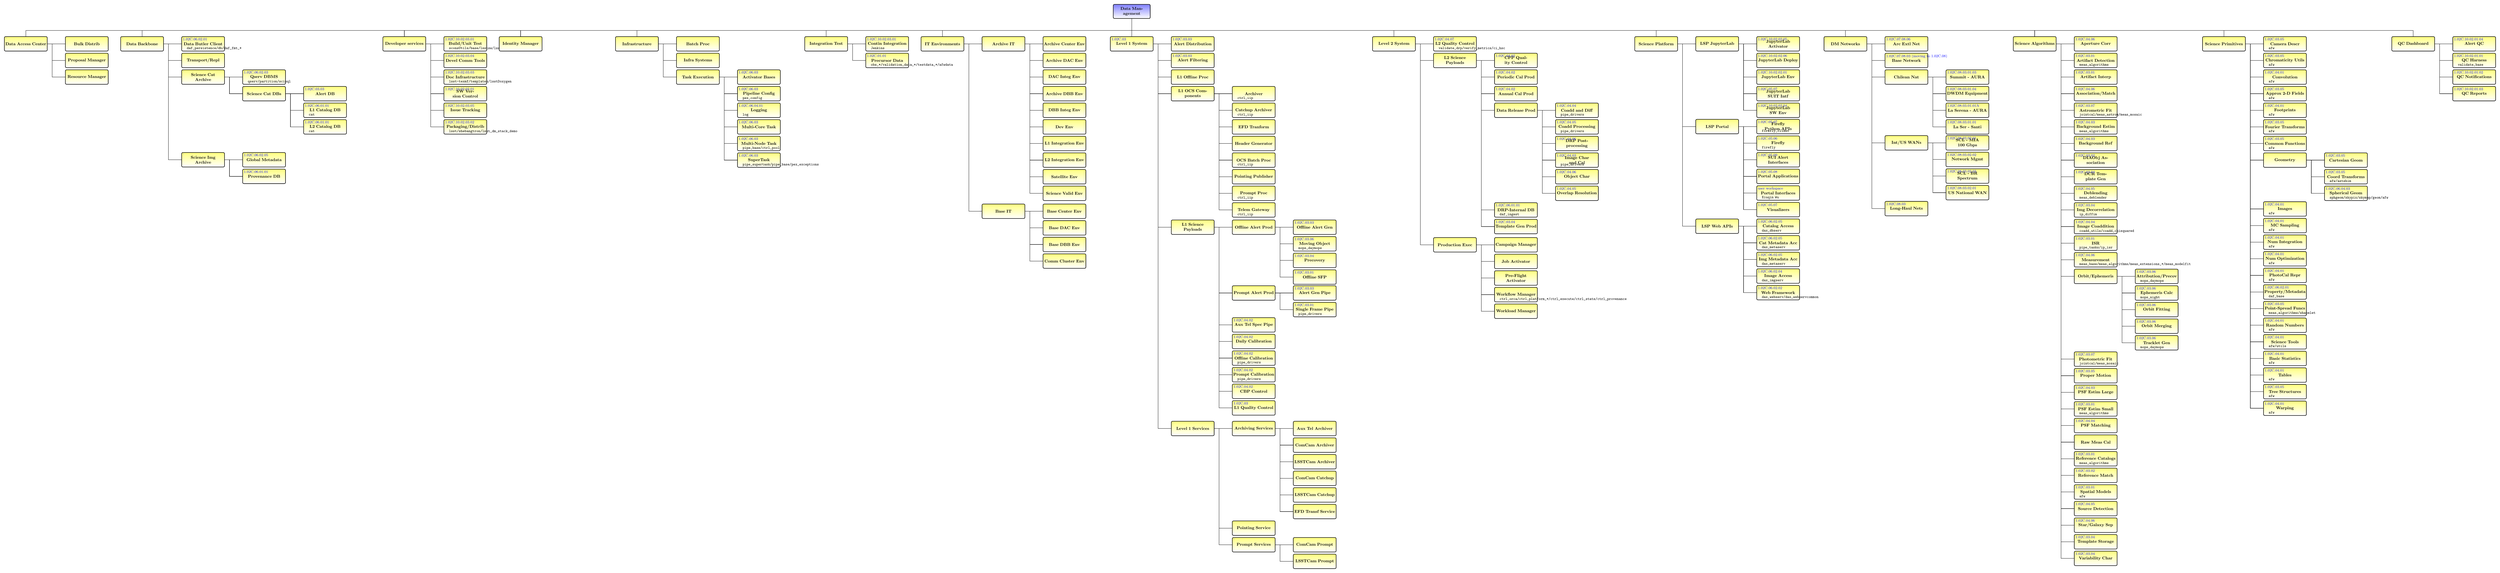
\begin{tikzpicture}[node distance=0mm]
\node (DAC) [pbox, 
] {\textbf{Data Access Center} };
\node [below right] at (DAC.north west) {\small \color{blue}.} ;
\node (BULKD) [pbox,right=15mm of DAC] {\textbf{Bulk Distrib} };
 \draw[pline] (DAC.east) -| ++(0.4,0) |- (BULKD.west); 
\node (DACPROP) [pbox,below=4pt of BULKD] {\textbf{Proposal Manager} };
 \draw[pline] (DAC.east) -| ++(0.4,0) |- (DACPROP.west); 
\node (DACRM) [pbox,below=4pt of DACPROP] {\textbf{Resource Manager} };
 \draw[pline] (DAC.east) -| ++(0.4,0) |- (DACRM.west); 
\node (DBB) [pbox, 
right=6.2cm of DAC] {\textbf{Data Backbone} };
\node [below right] at (DBB.north west) {\small \color{blue}.} ;
\node (BUTLER) [pbox,right=15mm of DBB] {\textbf{Data Butler Client} };
\node [below right] at (BUTLER.north west) {\small \color{blue}1.02C.06.02.01} ;
\node (BUTLERpkg) [tbox,below=3mm of BUTLER.north] {{\small \color{black} \begin{verbatim} daf_persistence/db/daf_fmt_* \end{verbatim} }  };
 \draw[pline] (DBB.east) -| ++(0.4,0) |- (BUTLER.west); 
\node (DTR) [pbox,below=4pt of BUTLER] {\textbf{Transport/Repl} };
 \draw[pline] (DBB.east) -| ++(0.4,0) |- (DTR.west); 
\node (SCICATAR) [pbox,below=4pt of DTR] {\textbf{Science Cat Archive} };
\node [below right] at (SCICATAR.north west) {\small \color{blue}.} ;
 \draw[pline] (DBB.east) -| ++(0.4,0) |- (SCICATAR.west); 
\node (QSERV) [pbox,right=15mm of SCICATAR] {\textbf{Qserv DBMS} };
\node [below right] at (QSERV.north west) {\small \color{blue}1.02C.06.02.03} ;
\node (QSERVpkg) [tbox,below=3mm of QSERV.north] {{\small \color{black} \begin{verbatim} qserv/partition/scisql \end{verbatim} }  };
 \draw[pline] (SCICATAR.east) -| ++(0.4,0) |- (QSERV.west); 
\node (SCICATDB) [pbox,below=4pt of QSERV] {\textbf{Science Cat DBs} };
\node [below right] at (SCICATDB.north west) {\small \color{blue}.} ;
 \draw[pline] (SCICATAR.east) -| ++(0.4,0) |- (SCICATDB.west); 
\node (ALERTDB) [pbox,right=15mm of SCICATDB] {\textbf{Alert DB} };
\node [below right] at (ALERTDB.north west) {\small \color{blue}1.02C.03.03} ;
 \draw[pline] (SCICATDB.east) -| ++(0.4,0) |- (ALERTDB.west); 
\node (L1DB) [pbox,below=4pt of ALERTDB] {\textbf{L1 Catalog DB} };
\node [below right] at (L1DB.north west) {\small \color{blue}1.02C.06.01.01} ;
\node (L1DBpkg) [tbox,below=3mm of L1DB.north] {{\small \color{black} \begin{verbatim} cat \end{verbatim} }  };
 \draw[pline] (SCICATDB.east) -| ++(0.4,0) |- (L1DB.west); 
\node (L2DB) [pbox,below=4pt of L1DB] {\textbf{L2 Catalog DB} };
\node [below right] at (L2DB.north west) {\small \color{blue}1.02C.06.01.01} ;
\node (L2DBpkg) [tbox,below=3mm of L2DB.north] {{\small \color{black} \begin{verbatim} cat \end{verbatim} }  };
 \draw[pline] (SCICATDB.east) -| ++(0.4,0) |- (L2DB.west); 
\node (SCIIMGAR) [pbox,below=164pt of SCICATAR] {\textbf{Science Img Archive} };
\node [below right] at (SCIIMGAR.north west) {\small \color{blue}.} ;
 \draw[pline] (DBB.east) -| ++(0.4,0) |- (SCIIMGAR.west); 
\node (GMDS) [pbox,right=15mm of SCIIMGAR] {\textbf{Global Metadata} };
\node [below right] at (GMDS.north west) {\small \color{blue}1.02C.06.02.05} ;
 \draw[pline] (SCIIMGAR.east) -| ++(0.4,0) |- (GMDS.west); 
\node (PRVDB) [pbox,below=4pt of GMDS] {\textbf{Provenance DB} };
\node [below right] at (PRVDB.north west) {\small \color{blue}1.02C.06.01.01} ;
 \draw[pline] (SCIIMGAR.east) -| ++(0.4,0) |- (PRVDB.west); 
\node (DEVEL) [pbox, 
right=18.6cm of DBB] {\textbf{Developer services} };
\node [below right] at (DEVEL.north west) {\small \color{blue}.} ;
\node (BUILD) [pbox,right=15mm of DEVEL] {\textbf{Build/Unit Test} };
\node [below right] at (BUILD.north west) {\small \color{blue}1.02C.10.02.03.01} ;
\node (BUILDpkg) [tbox,below=3mm of BUILD.north] {{\small \color{black} \begin{verbatim} sconsUtils/base/lsstsw/lsst_build \end{verbatim} }  };
 \draw[pline] (DEVEL.east) -| ++(0.4,0) |- (BUILD.west); 
\node (COMMS) [pbox,below=4pt of BUILD] {\textbf{Devel Comm Tools} };
\node [below right] at (COMMS.north west) {\small \color{blue}1.02C.10.02.03.04} ;
 \draw[pline] (DEVEL.east) -| ++(0.4,0) |- (COMMS.west); 
\node (DOCS) [pbox,below=4pt of COMMS] {\textbf{Doc Infrastructure} };
\node [below right] at (DOCS.north west) {\small \color{blue}1.02C.10.02.03.03} ;
\node (DOCSpkg) [tbox,below=3mm of DOCS.north] {{\small \color{black} \begin{verbatim} lsst-texmf/templates/lsstDoxygen \end{verbatim} }  };
 \draw[pline] (DEVEL.east) -| ++(0.4,0) |- (DOCS.west); 
\node (DVCS) [pbox,below=4pt of DOCS] {\textbf{SW Version Control} };
\node [below right] at (DVCS.north west) {\small \color{blue}1.02C.10.02.03.01} ;
 \draw[pline] (DEVEL.east) -| ++(0.4,0) |- (DVCS.west); 
\node (ISSUE) [pbox,below=4pt of DVCS] {\textbf{Issue Tracking} };
\node [below right] at (ISSUE.north west) {\small \color{blue}1.02C.10.02.03.05} ;
 \draw[pline] (DEVEL.east) -| ++(0.4,0) |- (ISSUE.west); 
\node (PKG) [pbox,below=4pt of ISSUE] {\textbf{Packaging/Distrib} };
\node [below right] at (PKG.north west) {\small \color{blue}1.02C.10.02.03.02} ;
\node (PKGpkg) [tbox,below=3mm of PKG.north] {{\small \color{black} \begin{verbatim} lsst/shebangtron/lsst_dm_stack_demo \end{verbatim} }  };
 \draw[pline] (DEVEL.east) -| ++(0.4,0) |- (PKG.west); 
\node (IDM) [pbox, 
right=6.2cm of DEVEL] {\textbf{Identity Manager} };
\node (INFRA) [pbox, 
right=6.2cm of IDM] {\textbf{Infrastructure} };
\node [below right] at (INFRA.north west) {\small \color{blue}.} ;
\node (BPS) [pbox,right=15mm of INFRA] {\textbf{Batch Proc} };
 \draw[pline] (INFRA.east) -| ++(0.4,0) |- (BPS.west); 
\node (INFRASYS) [pbox,below=4pt of BPS] {\textbf{Infra Systems} };
 \draw[pline] (INFRA.east) -| ++(0.4,0) |- (INFRASYS.west); 
\node (TXF) [pbox,below=4pt of INFRASYS] {\textbf{Task Execution} };
\node [below right] at (TXF.north west) {\small \color{blue}.} ;
 \draw[pline] (INFRA.east) -| ++(0.4,0) |- (TXF.west); 
\node (ACTIVATR) [pbox,right=15mm of TXF] {\textbf{Activator Bases} };
\node [below right] at (ACTIVATR.north west) {\small \color{blue}1.02C.06.03} ;
 \draw[pline] (TXF.east) -| ++(0.4,0) |- (ACTIVATR.west); 
\node (CONFIG) [pbox,below=4pt of ACTIVATR] {\textbf{Pipeline Config} };
\node [below right] at (CONFIG.north west) {\small \color{blue}1.02C.06.03} ;
\node (CONFIGpkg) [tbox,below=3mm of CONFIG.north] {{\small \color{black} \begin{verbatim} pex_config \end{verbatim} }  };
 \draw[pline] (TXF.east) -| ++(0.4,0) |- (CONFIG.west); 
\node (LOG) [pbox,below=4pt of CONFIG] {\textbf{Logging} };
\node [below right] at (LOG.north west) {\small \color{blue}1.02C.06.04.01} ;
\node (LOGpkg) [tbox,below=3mm of LOG.north] {{\small \color{black} \begin{verbatim} log \end{verbatim} }  };
 \draw[pline] (TXF.east) -| ++(0.4,0) |- (LOG.west); 
\node (MULTCORE) [pbox,below=4pt of LOG] {\textbf{Multi-Core Task} };
\node [below right] at (MULTCORE.north west) {\small \color{blue}1.02C.06.03} ;
 \draw[pline] (TXF.east) -| ++(0.4,0) |- (MULTCORE.west); 
\node (MULTNODE) [pbox,below=4pt of MULTCORE] {\textbf{Multi-Node Task} };
\node [below right] at (MULTNODE.north west) {\small \color{blue}1.02C.06.03} ;
\node (MULTNODEpkg) [tbox,below=3mm of MULTNODE.north] {{\small \color{black} \begin{verbatim} pipe_base/ctrl_pool \end{verbatim} }  };
 \draw[pline] (TXF.east) -| ++(0.4,0) |- (MULTNODE.west); 
\node (SPRTASK) [pbox,below=4pt of MULTNODE] {\textbf{SuperTask} };
\node [below right] at (SPRTASK.north west) {\small \color{blue}1.02C.06.03} ;
\node (SPRTASKpkg) [tbox,below=3mm of SPRTASK.north] {{\small \color{black} \begin{verbatim} pipe_supertask/pipe_base/pex_exceptions \end{verbatim} }  };
 \draw[pline] (TXF.east) -| ++(0.4,0) |- (SPRTASK.west); 
\node (INTGTEST) [pbox, 
right=12.4cm of INFRA] {\textbf{Integration Test} };
\node [below right] at (INTGTEST.north west) {\small \color{blue}.} ;
\node (CI) [pbox,right=15mm of INTGTEST] {\textbf{Contin Integration} };
\node [below right] at (CI.north west) {\small \color{blue}1.02C.10.02.03.01} ;
\node (CIpkg) [tbox,below=3mm of CI.north] {{\small \color{black} \begin{verbatim} Jenkins \end{verbatim} }  };
 \draw[pline] (INTGTEST.east) -| ++(0.4,0) |- (CI.west); 
\node (PRECURSR) [pbox,below=4pt of CI] {\textbf{Precursor Data} };
\node [below right] at (PRECURSR.north west) {\small \color{blue}1.02C.01.01} ;
\node (PRECURSRpkg) [tbox,below=3mm of PRECURSR.north] {{\small \color{black} \begin{verbatim} obs_*/validation_data_*/testdata_*/afwdata \end{verbatim} }  };
 \draw[pline] (INTGTEST.east) -| ++(0.4,0) |- (PRECURSR.west); 
\node (ITENV) [pbox, 
right=6.2cm of INTGTEST] {\textbf{IT Environments} };
\node [below right] at (ITENV.north west) {\small \color{blue}.} ;
\node (ITARC) [pbox,right=15mm of ITENV] {\textbf{Archive IT} };
\node [below right] at (ITARC.north west) {\small \color{blue}.} ;
 \draw[pline] (ITENV.east) -| ++(0.4,0) |- (ITARC.west); 
\node (CTRENV) [pbox,right=15mm of ITARC] {\textbf{Archive Center Env} };
 \draw[pline] (ITARC.east) -| ++(0.4,0) |- (CTRENV.west); 
\node (DACENV) [pbox,below=4pt of CTRENV] {\textbf{Archive DAC Env} };
 \draw[pline] (ITARC.east) -| ++(0.4,0) |- (DACENV.west); 
\node (DACINTGR) [pbox,below=4pt of DACENV] {\textbf{DAC Integ Env} };
 \draw[pline] (ITARC.east) -| ++(0.4,0) |- (DACINTGR.west); 
\node (DBBENV) [pbox,below=4pt of DACINTGR] {\textbf{Archive DBB Env} };
 \draw[pline] (ITARC.east) -| ++(0.4,0) |- (DBBENV.west); 
\node (DBBINTGR) [pbox,below=4pt of DBBENV] {\textbf{DBB Integ Env} };
 \draw[pline] (ITARC.east) -| ++(0.4,0) |- (DBBINTGR.west); 
\node (DEVENV) [pbox,below=4pt of DBBINTGR] {\textbf{Dev Env} };
 \draw[pline] (ITARC.east) -| ++(0.4,0) |- (DEVENV.west); 
\node (L1INTGR) [pbox,below=4pt of DEVENV] {\textbf{L1 Integration Env} };
 \draw[pline] (ITARC.east) -| ++(0.4,0) |- (L1INTGR.west); 
\node (L2INTGR) [pbox,below=4pt of L1INTGR] {\textbf{L2 Integration Env} };
 \draw[pline] (ITARC.east) -| ++(0.4,0) |- (L2INTGR.west); 
\node (SATENV) [pbox,below=4pt of L2INTGR] {\textbf{Satellite Env} };
 \draw[pline] (ITARC.east) -| ++(0.4,0) |- (SATENV.west); 
\node (SVENV) [pbox,below=4pt of SATENV] {\textbf{Science Valid Env} };
 \draw[pline] (ITARC.east) -| ++(0.4,0) |- (SVENV.west); 
\node (ITBASE) [pbox,below=369pt of ITARC] {\textbf{Base IT} };
\node [below right] at (ITBASE.north west) {\small \color{blue}.} ;
 \draw[pline] (ITENV.east) -| ++(0.4,0) |- (ITBASE.west); 
\node (BCTRENV) [pbox,right=15mm of ITBASE] {\textbf{Base Center Env} };
 \draw[pline] (ITBASE.east) -| ++(0.4,0) |- (BCTRENV.west); 
\node (BDACENV) [pbox,below=4pt of BCTRENV] {\textbf{Base DAC Env} };
 \draw[pline] (ITBASE.east) -| ++(0.4,0) |- (BDACENV.west); 
\node (BDBBENV) [pbox,below=4pt of BDACENV] {\textbf{Base DBB Env} };
 \draw[pline] (ITBASE.east) -| ++(0.4,0) |- (BDBBENV.west); 
\node (COMMENV) [pbox,below=4pt of BDBBENV] {\textbf{Comm Cluster Env} };
 \draw[pline] (ITBASE.east) -| ++(0.4,0) |- (COMMENV.west); 
\node (L1) [pbox, 
right=12.4cm of ITENV] {\textbf{Level 1 System} };
\node [below right] at (L1.north west) {\small \color{blue}1.02C.03} ;
\node (ALRTDSTR) [pbox,right=15mm of L1] {\textbf{Alert Distribution} };
\node [below right] at (ALRTDSTR.north west) {\small \color{blue}1.02C.03.03} ;
 \draw[pline] (L1.east) -| ++(0.4,0) |- (ALRTDSTR.west); 
\node (ALRTFLTR) [pbox,below=4pt of ALRTDSTR] {\textbf{Alert Filtering} };
\node [below right] at (ALRTFLTR.north west) {\small \color{blue}1.02C.03.03} ;
 \draw[pline] (L1.east) -| ++(0.4,0) |- (ALRTFLTR.west); 
\node (L1OFFL) [pbox,below=4pt of ALRTFLTR] {\textbf{L1 Offline Proc} };
 \draw[pline] (L1.east) -| ++(0.4,0) |- (L1OFFL.west); 
\node (L1ONL) [pbox,below=4pt of L1OFFL] {\textbf{L1 OCS Components} };
\node [below right] at (L1ONL.north west) {\small \color{blue}.} ;
 \draw[pline] (L1.east) -| ++(0.4,0) |- (L1ONL.west); 
\node (ARC) [pbox,right=15mm of L1ONL] {\textbf{Archiver} };
\node (ARCpkg) [tbox,below=3mm of ARC.north] {{\small \color{black} \begin{verbatim} ctrl_iip \end{verbatim} }  };
 \draw[pline] (L1ONL.east) -| ++(0.4,0) |- (ARC.west); 
\node (CARC) [pbox,below=4pt of ARC] {\textbf{Catchup Archiver} };
\node (CARCpkg) [tbox,below=3mm of CARC.north] {{\small \color{black} \begin{verbatim} ctrl_iip \end{verbatim} }  };
 \draw[pline] (L1ONL.east) -| ++(0.4,0) |- (CARC.west); 
\node (EFDT) [pbox,below=4pt of CARC] {\textbf{EFD Tranform} };
 \draw[pline] (L1ONL.east) -| ++(0.4,0) |- (EFDT.west); 
\node (HEADER) [pbox,below=4pt of EFDT] {\textbf{Header Generator} };
 \draw[pline] (L1ONL.east) -| ++(0.4,0) |- (HEADER.west); 
\node (OCSBAT) [pbox,below=4pt of HEADER] {\textbf{OCS Batch Proc} };
\node (OCSBATpkg) [tbox,below=3mm of OCSBAT.north] {{\small \color{black} \begin{verbatim} ctrl_iip \end{verbatim} }  };
 \draw[pline] (L1ONL.east) -| ++(0.4,0) |- (OCSBAT.west); 
\node (POINTP) [pbox,below=4pt of OCSBAT] {\textbf{Pointing Publisher} };
 \draw[pline] (L1ONL.east) -| ++(0.4,0) |- (POINTP.west); 
\node (PRMPT) [pbox,below=4pt of POINTP] {\textbf{Prompt Proc} };
\node (PRMPTpkg) [tbox,below=3mm of PRMPT.north] {{\small \color{black} \begin{verbatim} ctrl_iip \end{verbatim} }  };
 \draw[pline] (L1ONL.east) -| ++(0.4,0) |- (PRMPT.west); 
\node (TMG) [pbox,below=4pt of PRMPT] {\textbf{Telem Gateway} };
\node (TMGpkg) [tbox,below=3mm of TMG.north] {{\small \color{black} \begin{verbatim} ctrl_iip \end{verbatim} }  };
 \draw[pline] (L1ONL.east) -| ++(0.4,0) |- (TMG.west); 
\node (L1SCI) [pbox,below=287pt of L1ONL] {\textbf{L1 Science Payloads} };
\node [below right] at (L1SCI.north west) {\small \color{blue}.} ;
 \draw[pline] (L1.east) -| ++(0.4,0) |- (L1SCI.west); 
\node (APOFFL) [pbox,right=15mm of L1SCI] {\textbf{Offline Alert Prod} };
\node [below right] at (APOFFL.north west) {\small \color{blue}.} ;
 \draw[pline] (L1SCI.east) -| ++(0.4,0) |- (APOFFL.west); 
\node (ALRTOFFL) [pbox,right=15mm of APOFFL] {\textbf{Offline Alert Gen} };
\node [below right] at (ALRTOFFL.north west) {\small \color{blue}1.02C.03.03} ;
 \draw[pline] (APOFFL.east) -| ++(0.4,0) |- (ALRTOFFL.west); 
\node (MOPS) [pbox,below=4pt of ALRTOFFL] {\textbf{Moving Object} };
\node [below right] at (MOPS.north west) {\small \color{blue}1.02C.03.06} ;
\node (MOPSpkg) [tbox,below=3mm of MOPS.north] {{\small \color{black} \begin{verbatim} mops_daymops \end{verbatim} }  };
 \draw[pline] (APOFFL.east) -| ++(0.4,0) |- (MOPS.west); 
\node (PRECOV) [pbox,below=4pt of MOPS] {\textbf{Precovery} };
\node [below right] at (PRECOV.north west) {\small \color{blue}1.02C.03.04} ;
 \draw[pline] (APOFFL.east) -| ++(0.4,0) |- (PRECOV.west); 
\node (SFPOFFL) [pbox,below=4pt of PRECOV] {\textbf{Offline SFP} };
\node [below right] at (SFPOFFL.north west) {\small \color{blue}1.02C.03.01} ;
 \draw[pline] (APOFFL.east) -| ++(0.4,0) |- (SFPOFFL.west); 
\node (APPRMPT) [pbox,below=123pt of APOFFL] {\textbf{Prompt Alert Prod} };
\node [below right] at (APPRMPT.north west) {\small \color{blue}.} ;
 \draw[pline] (L1SCI.east) -| ++(0.4,0) |- (APPRMPT.west); 
\node (ALERTPIPE) [pbox,right=15mm of APPRMPT] {\textbf{Alert Gen Pipe} };
\node [below right] at (ALERTPIPE.north west) {\small \color{blue}1.02C.03.03} ;
 \draw[pline] (APPRMPT.east) -| ++(0.4,0) |- (ALERTPIPE.west); 
\node (SFPPIPE) [pbox,below=4pt of ALERTPIPE] {\textbf{Single Frame Pipe} };
\node [below right] at (SFPPIPE.north west) {\small \color{blue}1.02C.03.01} ;
\node (SFPPIPEpkg) [tbox,below=3mm of SFPPIPE.north] {{\small \color{black} \begin{verbatim} pipe_drivers \end{verbatim} }  };
 \draw[pline] (APPRMPT.east) -| ++(0.4,0) |- (SFPPIPE.west); 
\node (AUXTEL) [pbox,below=41pt of APPRMPT] {\textbf{Aux Tel Spec Pipe} };
\node [below right] at (AUXTEL.north west) {\small \color{blue}1.02C.04.02} ;
 \draw[pline] (L1SCI.east) -| ++(0.4,0) |- (AUXTEL.west); 
\node (CALDAILY) [pbox,below=4pt of AUXTEL] {\textbf{Daily Calibration} };
\node [below right] at (CALDAILY.north west) {\small \color{blue}1.02C.04.02} ;
 \draw[pline] (L1SCI.east) -| ++(0.4,0) |- (CALDAILY.west); 
\node (CALOFFL) [pbox,below=4pt of CALDAILY] {\textbf{Offline Calibration} };
\node [below right] at (CALOFFL.north west) {\small \color{blue}1.02C.04.02} ;
\node (CALOFFLpkg) [tbox,below=3mm of CALOFFL.north] {{\small \color{black} \begin{verbatim} pipe_drivers \end{verbatim} }  };
 \draw[pline] (L1SCI.east) -| ++(0.4,0) |- (CALOFFL.west); 
\node (CALPRMPT) [pbox,below=4pt of CALOFFL] {\textbf{Prompt Calibration} };
\node [below right] at (CALPRMPT.north west) {\small \color{blue}1.02C.04.02} ;
\node (CALPRMPTpkg) [tbox,below=3mm of CALPRMPT.north] {{\small \color{black} \begin{verbatim} pipe_drivers \end{verbatim} }  };
 \draw[pline] (L1SCI.east) -| ++(0.4,0) |- (CALPRMPT.west); 
\node (CBPCTRL) [pbox,below=4pt of CALPRMPT] {\textbf{CBP Control} };
\node [below right] at (CBPCTRL.north west) {\small \color{blue}1.02C.04.02} ;
 \draw[pline] (L1SCI.east) -| ++(0.4,0) |- (CBPCTRL.west); 
\node (L1QC) [pbox,below=4pt of CBPCTRL] {\textbf{L1 Quality Control} };
\node [below right] at (L1QC.north west) {\small \color{blue}1.02C.03} ;
 \draw[pline] (L1SCI.east) -| ++(0.4,0) |- (L1QC.west); 
\node (L1SRV) [pbox,below=451pt of L1SCI] {\textbf{Level 1 Services} };
\node [below right] at (L1SRV.north west) {\small \color{blue}.} ;
 \draw[pline] (L1.east) -| ++(0.4,0) |- (L1SRV.west); 
\node (ARCSRV) [pbox,right=15mm of L1SRV] {\textbf{Archiving Services} };
\node [below right] at (ARCSRV.north west) {\small \color{blue}.} ;
 \draw[pline] (L1SRV.east) -| ++(0.4,0) |- (ARCSRV.west); 
\node (ARCAT) [pbox,right=15mm of ARCSRV] {\textbf{Aux Tel Archiver} };
 \draw[pline] (ARCSRV.east) -| ++(0.4,0) |- (ARCAT.west); 
\node (ARCCOM) [pbox,below=4pt of ARCAT] {\textbf{ComCam Archiver} };
 \draw[pline] (ARCSRV.east) -| ++(0.4,0) |- (ARCCOM.west); 
\node (ARCLSST) [pbox,below=4pt of ARCCOM] {\textbf{LSSTCam Archiver} };
 \draw[pline] (ARCSRV.east) -| ++(0.4,0) |- (ARCLSST.west); 
\node (CARCCOM) [pbox,below=4pt of ARCLSST] {\textbf{ComCam Catchup} };
 \draw[pline] (ARCSRV.east) -| ++(0.4,0) |- (CARCCOM.west); 
\node (CARCLSST) [pbox,below=4pt of CARCCOM] {\textbf{LSSTCam Catchup} };
 \draw[pline] (ARCSRV.east) -| ++(0.4,0) |- (CARCLSST.west); 
\node (EFDTSRV) [pbox,below=4pt of CARCLSST] {\textbf{EFD Transf Service} };
 \draw[pline] (ARCSRV.east) -| ++(0.4,0) |- (EFDTSRV.west); 
\node (POINTSRV) [pbox,below=205pt of ARCSRV] {\textbf{Pointing Service} };
 \draw[pline] (L1SRV.east) -| ++(0.4,0) |- (POINTSRV.west); 
\node (PRMPTSRV) [pbox,below=4pt of POINTSRV] {\textbf{Prompt Services} };
\node [below right] at (PRMPTSRV.north west) {\small \color{blue}.} ;
 \draw[pline] (L1SRV.east) -| ++(0.4,0) |- (PRMPTSRV.west); 
\node (PRMPTCOM) [pbox,right=15mm of PRMPTSRV] {\textbf{ComCam Prompt} };
 \draw[pline] (PRMPTSRV.east) -| ++(0.4,0) |- (PRMPTCOM.west); 
\node (PRMPTLSST) [pbox,below=4pt of PRMPTCOM] {\textbf{LSSTCam Prompt} };
 \draw[pline] (PRMPTSRV.east) -| ++(0.4,0) |- (PRMPTLSST.west); 
\node (L2) [pbox, 
right=18.6cm of L1] {\textbf{Level 2 System} };
\node [below right] at (L2.north west) {\small \color{blue}.} ;
\node (L2QC) [pbox,right=15mm of L2] {\textbf{L2 Quality Control} };
\node [below right] at (L2QC.north west) {\small \color{blue}1.02C.04.07} ;
\node (L2QCpkg) [tbox,below=3mm of L2QC.north] {{\small \color{black} \begin{verbatim} validate_drp/verify_metrics/ci_hsc \end{verbatim} }  };
 \draw[pline] (L2.east) -| ++(0.4,0) |- (L2QC.west); 
\node (L2SCI) [pbox,below=4pt of L2QC] {\textbf{L2 Science Payloads} };
\node [below right] at (L2SCI.north west) {\small \color{blue}.} ;
 \draw[pline] (L2.east) -| ++(0.4,0) |- (L2SCI.west); 
\node (CPPQC) [pbox,right=15mm of L2SCI] {\textbf{CPP Quality Control} };
\node [below right] at (CPPQC.north west) {\small \color{blue}1.02C.04.02} ;
 \draw[pline] (L2SCI.east) -| ++(0.4,0) |- (CPPQC.west); 
\node (CPPSLOW) [pbox,below=4pt of CPPQC] {\textbf{Periodic Cal Prod} };
\node [below right] at (CPPSLOW.north west) {\small \color{blue}1.02C.04.02} ;
 \draw[pline] (L2SCI.east) -| ++(0.4,0) |- (CPPSLOW.west); 
\node (CPPYEAR) [pbox,below=4pt of CPPSLOW] {\textbf{Annual Cal Prod} };
\node [below right] at (CPPYEAR.north west) {\small \color{blue}1.02C.04.02} ;
 \draw[pline] (L2SCI.east) -| ++(0.4,0) |- (CPPYEAR.west); 
\node (DRP) [pbox,below=4pt of CPPYEAR] {\textbf{Data Release Prod} };
\node [below right] at (DRP.north west) {\small \color{blue}.} ;
 \draw[pline] (L2SCI.east) -| ++(0.4,0) |- (DRP.west); 
\node (COADPIPE) [pbox,right=15mm of DRP] {\textbf{Coadd and Diff} };
\node [below right] at (COADPIPE.north west) {\small \color{blue}1.02C.04.04} ;
\node (COADPIPEpkg) [tbox,below=3mm of COADPIPE.north] {{\small \color{black} \begin{verbatim} pipe_drivers \end{verbatim} }  };
 \draw[pline] (DRP.east) -| ++(0.4,0) |- (COADPIPE.west); 
\node (COADPROC) [pbox,below=4pt of COADPIPE] {\textbf{Coadd Processing} };
\node [below right] at (COADPROC.north west) {\small \color{blue}1.02C.04.05} ;
\node (COADPROCpkg) [tbox,below=3mm of COADPROC.north] {{\small \color{black} \begin{verbatim} pipe_drivers \end{verbatim} }  };
 \draw[pline] (DRP.east) -| ++(0.4,0) |- (COADPROC.west); 
\node (DRPPOST) [pbox,below=4pt of COADPROC] {\textbf{DRP Postprocessing} };
\node [below right] at (DRPPOST.north west) {\small \color{blue}1.02C.04.06} ;
 \draw[pline] (DRP.east) -| ++(0.4,0) |- (DRPPOST.west); 
\node (IMGCHAR) [pbox,below=4pt of DRPPOST] {\textbf{Image Char and Cal} };
\node [below right] at (IMGCHAR.north west) {\small \color{blue}1.02C.04.03} ;
\node (IMGCHARpkg) [tbox,below=3mm of IMGCHAR.north] {{\small \color{black} \begin{verbatim} pipe_drivers \end{verbatim} }  };
 \draw[pline] (DRP.east) -| ++(0.4,0) |- (IMGCHAR.west); 
\node (MULTIFIT) [pbox,below=4pt of IMGCHAR] {\textbf{Object Char} };
\node [below right] at (MULTIFIT.north west) {\small \color{blue}1.02C.04.06} ;
 \draw[pline] (DRP.east) -| ++(0.4,0) |- (MULTIFIT.west); 
\node (OVERLAP) [pbox,below=4pt of MULTIFIT] {\textbf{Overlap Resolution} };
\node [below right] at (OVERLAP.north west) {\small \color{blue}1.02C.04.05} ;
 \draw[pline] (DRP.east) -| ++(0.4,0) |- (OVERLAP.west); 
\node (DRPDB) [pbox,below=205pt of DRP] {\textbf{DRP-Internal DB} };
\node [below right] at (DRPDB.north west) {\small \color{blue}1.02C.06.01.01} ;
\node (DRPDBpkg) [tbox,below=3mm of DRPDB.north] {{\small \color{black} \begin{verbatim} daf_ingest \end{verbatim} }  };
 \draw[pline] (L2SCI.east) -| ++(0.4,0) |- (DRPDB.west); 
\node (TMPLGEN) [pbox,below=4pt of DRPDB] {\textbf{Template Gen Prod} };
\node [below right] at (TMPLGEN.north west) {\small \color{blue}1.02C.03.04} ;
 \draw[pline] (L2SCI.east) -| ++(0.4,0) |- (TMPLGEN.west); 
\node (PRODEX) [pbox,below=410pt of L2SCI] {\textbf{Production Exec} };
\node [below right] at (PRODEX.north west) {\small \color{blue}.} ;
 \draw[pline] (L2.east) -| ++(0.4,0) |- (PRODEX.west); 
\node (CMPGN) [pbox,right=15mm of PRODEX] {\textbf{Campaign Manager} };
 \draw[pline] (PRODEX.east) -| ++(0.4,0) |- (CMPGN.west); 
\node (JOBACTIV) [pbox,below=4pt of CMPGN] {\textbf{Job Activator} };
 \draw[pline] (PRODEX.east) -| ++(0.4,0) |- (JOBACTIV.west); 
\node (PREACTIV) [pbox,below=4pt of JOBACTIV] {\textbf{Pre-Flight Activator} };
 \draw[pline] (PRODEX.east) -| ++(0.4,0) |- (PREACTIV.west); 
\node (WFM) [pbox,below=4pt of PREACTIV] {\textbf{Workflow Manager} };
\node (WFMpkg) [tbox,below=3mm of WFM.north] {{\small \color{black} \begin{verbatim} ctrl_orca/ctrl_platform_*/ctrl_execute/ctrl_stats/ctrl_provenance \end{verbatim} }  };
 \draw[pline] (PRODEX.east) -| ++(0.4,0) |- (WFM.west); 
\node (WLM) [pbox,below=4pt of WFM] {\textbf{Workload Manager} };
 \draw[pline] (PRODEX.east) -| ++(0.4,0) |- (WLM.west); 
\node (LSP) [pbox, 
right=18.6cm of L2] {\textbf{Science Platform} };
\node [below right] at (LSP.north west) {\small \color{blue}.} ;
\node (LSPJL) [pbox,right=15mm of LSP] {\textbf{LSP JupyterLab} };
\node [below right] at (LSPJL.north west) {\small \color{blue}.} ;
 \draw[pline] (LSP.east) -| ++(0.4,0) |- (LSPJL.west); 
\node (JLACTIV) [pbox,right=15mm of LSPJL] {\textbf{JupyterLab Activator} };
\node [below right] at (JLACTIV.north west) {\small \color{blue}1.02C.10.02.02.05} ;
 \draw[pline] (LSPJL.east) -| ++(0.4,0) |- (JLACTIV.west); 
\node (JLDPLY) [pbox,below=4pt of JLACTIV] {\textbf{JupyterLab Deploy} };
\node [below right] at (JLDPLY.north west) {\small \color{blue}1.02C.10.02.02.06} ;
 \draw[pline] (LSPJL.east) -| ++(0.4,0) |- (JLDPLY.west); 
\node (JLENV) [pbox,below=4pt of JLDPLY] {\textbf{JupyterLab Env} };
\node [below right] at (JLENV.north west) {\small \color{blue}1.02C.10.02.02.01} ;
 \draw[pline] (LSPJL.east) -| ++(0.4,0) |- (JLENV.west); 
\node (JLSUIT) [pbox,below=4pt of JLENV] {\textbf{JupyterLab SUIT Intf} };
\node [below right] at (JLSUIT.north west) {\small \color{blue}1.02C.05.07} ;
 \draw[pline] (LSPJL.east) -| ++(0.4,0) |- (JLSUIT.west); 
\node (JLSW) [pbox,below=4pt of JLSUIT] {\textbf{JupyterLab SW Env} };
\node [below right] at (JLSW.north west) {\small \color{blue}1.02C.10.02.02.04} ;
 \draw[pline] (LSPJL.east) -| ++(0.4,0) |- (JLSW.west); 
\node (LSPPRTL) [pbox,below=164pt of LSPJL] {\textbf{LSP Portal} };
\node [below right] at (LSPPRTL.north west) {\small \color{blue}.} ;
 \draw[pline] (LSP.east) -| ++(0.4,0) |- (LSPPRTL.west); 
\node (FFLYAPI) [pbox,right=15mm of LSPPRTL] {\textbf{Firefly Python APIs} };
\node [below right] at (FFLYAPI.north west) {\small \color{blue}1.02C.05.07} ;
\node (FFLYAPIpkg) [tbox,below=3mm of FFLYAPI.north] {{\small \color{black} \begin{verbatim} firefly_client \end{verbatim} }  };
 \draw[pline] (LSPPRTL.east) -| ++(0.4,0) |- (FFLYAPI.west); 
\node (FIREFLY) [pbox,below=4pt of FFLYAPI] {\textbf{Firefly} };
\node [below right] at (FIREFLY.north west) {\small \color{blue}1.02C.05.06 } ;
\node (FIREFLYpkg) [tbox,below=3mm of FIREFLY.north] {{\small \color{black} \begin{verbatim} firefly \end{verbatim} }  };
 \draw[pline] (LSPPRTL.east) -| ++(0.4,0) |- (FIREFLY.west); 
\node (PRTLALRT) [pbox,below=4pt of FIREFLY] {\textbf{SUI Alert Interfaces} };
\node [below right] at (PRTLALRT.north west) {\small \color{blue}1.02C.05.09} ;
 \draw[pline] (LSPPRTL.east) -| ++(0.4,0) |- (PRTLALRT.west); 
\node (PRTLAPPS) [pbox,below=4pt of PRTLALRT] {\textbf{Portal Applications} };
\node [below right] at (PRTLAPPS.north west) {\small \color{blue}1.02C.05.08} ;
 \draw[pline] (LSPPRTL.east) -| ++(0.4,0) |- (PRTLAPPS.west); 
\node (PRTLINTF) [pbox,below=4pt of PRTLAPPS] {\textbf{Portal Interfaces} };
\node [below right] at (PRTLINTF.north west) {\small \color{blue} user workspace} ;
\node (PRTLINTFpkg) [tbox,below=3mm of PRTLINTF.north] {{\small \color{black} \begin{verbatim} Xiuqin Wu \end{verbatim} }  };
 \draw[pline] (LSPPRTL.east) -| ++(0.4,0) |- (PRTLINTF.west); 
\node (PRTLVIS) [pbox,below=4pt of PRTLINTF] {\textbf{Visualizers} };
\node [below right] at (PRTLVIS.north west) {\small \color{blue}1.02C.05.07} ;
 \draw[pline] (LSPPRTL.east) -| ++(0.4,0) |- (PRTLVIS.west); 
\node (LSPWEB) [pbox,below=205pt of LSPPRTL] {\textbf{LSP Web APIs} };
\node [below right] at (LSPWEB.north west) {\small \color{blue}.} ;
 \draw[pline] (LSP.east) -| ++(0.4,0) |- (LSPWEB.west); 
\node (DAXCAT) [pbox,right=15mm of LSPWEB] {\textbf{Catalog Access} };
\node [below right] at (DAXCAT.north west) {\small \color{blue}1.02C.06.02.05} ;
\node (DAXCATpkg) [tbox,below=3mm of DAXCAT.north] {{\small \color{black} \begin{verbatim} dax_dbserv \end{verbatim} }  };
 \draw[pline] (LSPWEB.east) -| ++(0.4,0) |- (DAXCAT.west); 
\node (DAXCMETA) [pbox,below=4pt of DAXCAT] {\textbf{Cat Metadata Acc} };
\node [below right] at (DAXCMETA.north west) {\small \color{blue}1.02C.06.02.05} ;
\node (DAXCMETApkg) [tbox,below=3mm of DAXCMETA.north] {{\small \color{black} \begin{verbatim} dax_metaserv \end{verbatim} }  };
 \draw[pline] (LSPWEB.east) -| ++(0.4,0) |- (DAXCMETA.west); 
\node (DAXIMETA) [pbox,below=4pt of DAXCMETA] {\textbf{Img Metadata Acc} };
\node [below right] at (DAXIMETA.north west) {\small \color{blue}1.02C.06.02.05} ;
\node (DAXIMETApkg) [tbox,below=3mm of DAXIMETA.north] {{\small \color{black} \begin{verbatim} dax_metaserv \end{verbatim} }  };
 \draw[pline] (LSPWEB.east) -| ++(0.4,0) |- (DAXIMETA.west); 
\node (DAXIMG) [pbox,below=4pt of DAXIMETA] {\textbf{Image Access} };
\node [below right] at (DAXIMG.north west) {\small \color{blue}1.02C.06.02.04} ;
\node (DAXIMGpkg) [tbox,below=3mm of DAXIMG.north] {{\small \color{black} \begin{verbatim} dax_imgserv \end{verbatim} }  };
 \draw[pline] (LSPWEB.east) -| ++(0.4,0) |- (DAXIMG.west); 
\node (DAXWEB) [pbox,below=4pt of DAXIMG] {\textbf{Web Framework} };
\node [below right] at (DAXWEB.north west) {\small \color{blue}1.02C.06.02.02} ;
\node (DAXWEBpkg) [tbox,below=3mm of DAXWEB.north] {{\small \color{black} \begin{verbatim} dax_webserv/dax_webservcommon \end{verbatim} }  };
 \draw[pline] (LSPWEB.east) -| ++(0.4,0) |- (DAXWEB.west); 
\node (NETDM) [pbox, 
right=12.4cm of LSP] {\textbf{DM Networks} };
\node [below right] at (NETDM.north west) {\small \color{blue}.} ;
\node (NETARCH) [pbox,right=15mm of NETDM] {\textbf{Arc Extl Net} };
\node [below right] at (NETARCH.north west) {\small \color{blue}1.02C.07.08.06} ;
 \draw[pline] (NETDM.east) -| ++(0.4,0) |- (NETARCH.west); 
\node (NETBASE) [pbox,below=4pt of NETARCH] {\textbf{Base Network} };
\node [below right] at (NETBASE.north west) {\small \color{blue}1.02C.07.08.03 (moving to 1.02C.08)} ;
 \draw[pline] (NETDM.east) -| ++(0.4,0) |- (NETBASE.west); 
\node (NETCHILE) [pbox,below=4pt of NETBASE] {\textbf{Chilean Nat} };
\node [below right] at (NETCHILE.north west) {\small \color{blue}.} ;
 \draw[pline] (NETDM.east) -| ++(0.4,0) |- (NETCHILE.west); 
\node (NETCPAG) [pbox,right=15mm of NETCHILE] {\textbf{Summit - AURA} };
\node [below right] at (NETCPAG.north west) {\small \color{blue}1.02C.08.03.01.03} ;
 \draw[pline] (NETCHILE.east) -| ++(0.4,0) |- (NETCPAG.west); 
\node (NETDWDM) [pbox,below=4pt of NETCPAG] {\textbf{DWDM Equipment} };
\node [below right] at (NETDWDM.north west) {\small \color{blue}1.02C.08.03.01.04} ;
 \draw[pline] (NETCHILE.east) -| ++(0.4,0) |- (NETDWDM.west); 
\node (NETLSAG) [pbox,below=4pt of NETDWDM] {\textbf{La Serena - AURA} };
\node [below right] at (NETLSAG.north west) {\small \color{blue}1.02C.08.03.01.01A} ;
 \draw[pline] (NETCHILE.east) -| ++(0.4,0) |- (NETLSAG.west); 
\node (NETLSSCL) [pbox,below=4pt of NETLSAG] {\textbf{La Ser - Santi } };
\node [below right] at (NETLSSCL.north west) {\small \color{blue}1.02C.08.03.01.01} ;
 \draw[pline] (NETCHILE.east) -| ++(0.4,0) |- (NETLSSCL.west); 
\node (NETINTLUS) [pbox,below=123pt of NETCHILE] {\textbf{Int/US WANs} };
\node [below right] at (NETINTLUS.north west) {\small \color{blue}.} ;
 \draw[pline] (NETDM.east) -| ++(0.4,0) |- (NETINTLUS.west); 
\node (NET100G) [pbox,right=15mm of NETINTLUS] {\textbf{SCL - MIA 100 Gbps } };
\node [below right] at (NET100G.north west) {\small \color{blue}1.02C.08.03.02.01} ;
 \draw[pline] (NETINTLUS.east) -| ++(0.4,0) |- (NET100G.west); 
\node (NETMGT) [pbox,below=4pt of NET100G] {\textbf{Network Mgmt} };
\node [below right] at (NETMGT.north west) {\small \color{blue}1.02C.08.03.02.02} ;
 \draw[pline] (NETINTLUS.east) -| ++(0.4,0) |- (NETMGT.west); 
\node (NETSPEC) [pbox,below=4pt of NETMGT] {\textbf{SCL - BR Spectrum } };
\node [below right] at (NETSPEC.north west) {\small \color{blue}1.02C.08.03.02.03} ;
 \draw[pline] (NETINTLUS.east) -| ++(0.4,0) |- (NETSPEC.west); 
\node (NETUSW) [pbox,below=4pt of NETSPEC] {\textbf{US National WAN} };
\node [below right] at (NETUSW.north west) {\small \color{blue}1.02C.08.03.02.01} ;
 \draw[pline] (NETINTLUS.east) -| ++(0.4,0) |- (NETUSW.west); 
\node (NETLHN) [pbox,below=123pt of NETINTLUS] {\textbf{Long-Haul Nets} };
\node [below right] at (NETLHN.north west) {\small \color{blue}1.02C.08.03} ;
 \draw[pline] (NETDM.east) -| ++(0.4,0) |- (NETLHN.west); 
\node (SCIALG) [pbox, 
right=12.4cm of NETDM] {\textbf{Science Algorithms} };
\node [below right] at (SCIALG.north west) {\small \color{blue}.} ;
\node (APCORR) [pbox,right=15mm of SCIALG] {\textbf{Aperture Corr} };
\node [below right] at (APCORR.north west) {\small \color{blue}1.02C.04.06} ;
 \draw[pline] (SCIALG.east) -| ++(0.4,0) |- (APCORR.west); 
\node (ARTFDET) [pbox,below=4pt of APCORR] {\textbf{Artifact Detection} };
\node [below right] at (ARTFDET.north west) {\small \color{blue}1.02C.03.01} ;
\node (ARTFDETpkg) [tbox,below=3mm of ARTFDET.north] {{\small \color{black} \begin{verbatim} meas_algorithms \end{verbatim} }  };
 \draw[pline] (SCIALG.east) -| ++(0.4,0) |- (ARTFDET.west); 
\node (ARTFINTP) [pbox,below=4pt of ARTFDET] {\textbf{Artifact Interp} };
\node [below right] at (ARTFINTP.north west) {\small \color{blue}1.02C.03.01} ;
 \draw[pline] (SCIALG.east) -| ++(0.4,0) |- (ARTFINTP.west); 
\node (ASSOC) [pbox,below=4pt of ARTFINTP] {\textbf{Association/Match} };
\node [below right] at (ASSOC.north west) {\small \color{blue}1.02C.04.06} ;
 \draw[pline] (SCIALG.east) -| ++(0.4,0) |- (ASSOC.west); 
\node (ASTROM) [pbox,below=4pt of ASSOC] {\textbf{Astrometric Fit} };
\node [below right] at (ASTROM.north west) {\small \color{blue}1.02C.03.07} ;
\node (ASTROMpkg) [tbox,below=3mm of ASTROM.north] {{\small \color{black} \begin{verbatim} jointcal/meas_astrom/meas_mosaic \end{verbatim} }  };
 \draw[pline] (SCIALG.east) -| ++(0.4,0) |- (ASTROM.west); 
\node (BKGDEST) [pbox,below=4pt of ASTROM] {\textbf{Background Estim} };
\node [below right] at (BKGDEST.north west) {\small \color{blue}1.02C.04.03} ;
\node (BKGDESTpkg) [tbox,below=3mm of BKGDEST.north] {{\small \color{black} \begin{verbatim} meas_algorithms \end{verbatim} }  };
 \draw[pline] (SCIALG.east) -| ++(0.4,0) |- (BKGDEST.west); 
\node (BKGDREF) [pbox,below=4pt of BKGDEST] {\textbf{Background Ref} };
\node [below right] at (BKGDREF.north west) {\small \color{blue}1.02C.04.03} ;
 \draw[pline] (SCIALG.east) -| ++(0.4,0) |- (BKGDREF.west); 
\node (DASSOC) [pbox,below=4pt of BKGDREF] {\textbf{DIAObj Association} };
\node [below right] at (DASSOC.north west) {\small \color{blue}1.02C.03.02} ;
 \draw[pline] (SCIALG.east) -| ++(0.4,0) |- (DASSOC.west); 
\node (DCRTMPL) [pbox,below=4pt of DASSOC] {\textbf{DCR Template Gen} };
\node [below right] at (DCRTMPL.north west) {\small \color{blue}1.02C.03.04} ;
 \draw[pline] (SCIALG.east) -| ++(0.4,0) |- (DCRTMPL.west); 
\node (DEBLEND) [pbox,below=4pt of DCRTMPL] {\textbf{Deblending} };
\node [below right] at (DEBLEND.north west) {\small \color{blue}1.02C.04.05} ;
\node (DEBLENDpkg) [tbox,below=3mm of DEBLEND.north] {{\small \color{black} \begin{verbatim} meas_deblender \end{verbatim} }  };
 \draw[pline] (SCIALG.east) -| ++(0.4,0) |- (DEBLEND.west); 
\node (DECORR) [pbox,below=4pt of DEBLEND] {\textbf{Img Decorrelation} };
\node [below right] at (DECORR.north west) {\small \color{blue}1.02C.03.04} ;
\node (DECORRpkg) [tbox,below=3mm of DECORR.north] {{\small \color{black} \begin{verbatim} ip_diffim \end{verbatim} }  };
 \draw[pline] (SCIALG.east) -| ++(0.4,0) |- (DECORR.west); 
\node (IMCOADD) [pbox,below=4pt of DECORR] {\textbf{Image Coaddition} };
\node [below right] at (IMCOADD.north west) {\small \color{blue}1.02C.04.04} ;
\node (IMCOADDpkg) [tbox,below=3mm of IMCOADD.north] {{\small \color{black} \begin{verbatim} coadd_utils/coadd_chisquared \end{verbatim} }  };
 \draw[pline] (SCIALG.east) -| ++(0.4,0) |- (IMCOADD.west); 
\node (ISR) [pbox,below=4pt of IMCOADD] {\textbf{ISR} };
\node [below right] at (ISR.north west) {\small \color{blue}1.02C.03.01} ;
\node (ISRpkg) [tbox,below=3mm of ISR.north] {{\small \color{black} \begin{verbatim} pipe_tasks/ip_isr \end{verbatim} }  };
 \draw[pline] (SCIALG.east) -| ++(0.4,0) |- (ISR.west); 
\node (MEASURE) [pbox,below=4pt of ISR] {\textbf{Measurement} };
\node [below right] at (MEASURE.north west) {\small \color{blue}1.02C.04.06} ;
\node (MEASUREpkg) [tbox,below=3mm of MEASURE.north] {{\small \color{black} \begin{verbatim} meas_base/meas_algorithms/meas_extensions_*/meas_modelfit \end{verbatim} }  };
 \draw[pline] (SCIALG.east) -| ++(0.4,0) |- (MEASURE.west); 
\node (ORBEP) [pbox,below=4pt of MEASURE] {\textbf{Orbit/Ephemeris} };
\node [below right] at (ORBEP.north west) {\small \color{blue}.} ;
 \draw[pline] (SCIALG.east) -| ++(0.4,0) |- (ORBEP.west); 
\node (ATTRIB) [pbox,right=15mm of ORBEP] {\textbf{Attribution/Precov} };
\node [below right] at (ATTRIB.north west) {\small \color{blue}1.02C.03.06} ;
\node (ATTRIBpkg) [tbox,below=3mm of ATTRIB.north] {{\small \color{black} \begin{verbatim} mops_daymops \end{verbatim} }  };
 \draw[pline] (ORBEP.east) -| ++(0.4,0) |- (ATTRIB.west); 
\node (EPHEM) [pbox,below=4pt of ATTRIB] {\textbf{Ephemeris Calc} };
\node [below right] at (EPHEM.north west) {\small \color{blue}1.02C.03.06} ;
\node (EPHEMpkg) [tbox,below=3mm of EPHEM.north] {{\small \color{black} \begin{verbatim} mops_night \end{verbatim} }  };
 \draw[pline] (ORBEP.east) -| ++(0.4,0) |- (EPHEM.west); 
\node (ORBFIT) [pbox,below=4pt of EPHEM] {\textbf{Orbit Fitting} };
\node [below right] at (ORBFIT.north west) {\small \color{blue}1.02C.03.06} ;
 \draw[pline] (ORBEP.east) -| ++(0.4,0) |- (ORBFIT.west); 
\node (ORBMERGE) [pbox,below=4pt of ORBFIT] {\textbf{Orbit Merging} };
\node [below right] at (ORBMERGE.north west) {\small \color{blue}1.02C.03.06} ;
 \draw[pline] (ORBEP.east) -| ++(0.4,0) |- (ORBMERGE.west); 
\node (TRACKLET) [pbox,below=4pt of ORBMERGE] {\textbf{Tracklet Gen} };
\node [below right] at (TRACKLET.north west) {\small \color{blue}1.02C.03.06} ;
\node (TRACKLETpkg) [tbox,below=3mm of TRACKLET.north] {{\small \color{black} \begin{verbatim} mops_daymops \end{verbatim} }  };
 \draw[pline] (ORBEP.east) -| ++(0.4,0) |- (TRACKLET.west); 
\node (PHOTOM) [pbox,below=164pt of ORBEP] {\textbf{Photometric Fit} };
\node [below right] at (PHOTOM.north west) {\small \color{blue}1.02C.03.07} ;
\node (PHOTOMpkg) [tbox,below=3mm of PHOTOM.north] {{\small \color{black} \begin{verbatim} jointcal/meas_mosaic \end{verbatim} }  };
 \draw[pline] (SCIALG.east) -| ++(0.4,0) |- (PHOTOM.west); 
\node (PRPRMOT) [pbox,below=4pt of PHOTOM] {\textbf{Proper Motion} };
\node [below right] at (PRPRMOT.north west) {\small \color{blue}1.02C.03.05} ;
 \draw[pline] (SCIALG.east) -| ++(0.4,0) |- (PRPRMOT.west); 
\node (PSFESTLG) [pbox,below=4pt of PRPRMOT] {\textbf{PSF Estim Large} };
\node [below right] at (PSFESTLG.north west) {\small \color{blue}1.02C.04.03} ;
 \draw[pline] (SCIALG.east) -| ++(0.4,0) |- (PSFESTLG.west); 
\node (PSFESTSM) [pbox,below=4pt of PSFESTLG] {\textbf{PSF Estim Small} };
\node [below right] at (PSFESTSM.north west) {\small \color{blue}1.02C.03.01} ;
\node (PSFESTSMpkg) [tbox,below=3mm of PSFESTSM.north] {{\small \color{black} \begin{verbatim} meas_algorithms \end{verbatim} }  };
 \draw[pline] (SCIALG.east) -| ++(0.4,0) |- (PSFESTSM.west); 
\node (PSFMATCH) [pbox,below=4pt of PSFESTSM] {\textbf{PSF Matching} };
\node [below right] at (PSFMATCH.north west) {\small \color{blue}1.02C.04.04} ;
 \draw[pline] (SCIALG.east) -| ++(0.4,0) |- (PSFMATCH.west); 
\node (RAWCAL) [pbox,below=4pt of PSFMATCH] {\textbf{Raw Meas Cal} };
 \draw[pline] (SCIALG.east) -| ++(0.4,0) |- (RAWCAL.west); 
\node (REFCAT) [pbox,below=4pt of RAWCAL] {\textbf{Reference Catalogs} };
\node [below right] at (REFCAT.north west) {\small \color{blue}1.02C.03.01} ;
\node (REFCATpkg) [tbox,below=3mm of REFCAT.north] {{\small \color{black} \begin{verbatim} meas_algorithms \end{verbatim} }  };
 \draw[pline] (SCIALG.east) -| ++(0.4,0) |- (REFCAT.west); 
\node (REFMATCH) [pbox,below=4pt of REFCAT] {\textbf{Reference Match} };
\node [below right] at (REFMATCH.north west) {\small \color{blue}1.02C.03.02} ;
 \draw[pline] (SCIALG.east) -| ++(0.4,0) |- (REFMATCH.west); 
\node (SPATMOD) [pbox,below=4pt of REFMATCH] {\textbf{Spatial Models} };
\node [below right] at (SPATMOD.north west) {\small \color{blue}1.02C.03.01} ;
\node (SPATMODpkg) [tbox,below=3mm of SPATMOD.north] {{\small \color{black} \begin{verbatim} afw \end{verbatim} }  };
 \draw[pline] (SCIALG.east) -| ++(0.4,0) |- (SPATMOD.west); 
\node (SRCDET) [pbox,below=4pt of SPATMOD] {\textbf{Source Detection} };
\node [below right] at (SRCDET.north west) {\small \color{blue}1.02C.04.05} ;
 \draw[pline] (SCIALG.east) -| ++(0.4,0) |- (SRCDET.west); 
\node (STARGAL) [pbox,below=4pt of SRCDET] {\textbf{Star/Galaxy Sep} };
\node [below right] at (STARGAL.north west) {\small \color{blue}1.02C.04.06} ;
 \draw[pline] (SCIALG.east) -| ++(0.4,0) |- (STARGAL.west); 
\node (TEMPLATE) [pbox,below=4pt of STARGAL] {\textbf{Template Storage} };
\node [below right] at (TEMPLATE.north west) {\small \color{blue}1.02C.03.04} ;
 \draw[pline] (SCIALG.east) -| ++(0.4,0) |- (TEMPLATE.west); 
\node (VRBLTY) [pbox,below=4pt of TEMPLATE] {\textbf{Variability Char} };
\node [below right] at (VRBLTY.north west) {\small \color{blue}1.02C.03.04} ;
 \draw[pline] (SCIALG.east) -| ++(0.4,0) |- (VRBLTY.west); 
\node (SCIPRIM) [pbox, 
right=12.4cm of SCIALG] {\textbf{Science Primitives} };
\node [below right] at (SCIPRIM.north west) {\small \color{blue}.} ;
\node (CAMDESC) [pbox,right=15mm of SCIPRIM] {\textbf{Camera Descr} };
\node [below right] at (CAMDESC.north west) {\small \color{blue}1.02C.03.05} ;
\node (CAMDESCpkg) [tbox,below=3mm of CAMDESC.north] {{\small \color{black} \begin{verbatim} afw \end{verbatim} }  };
 \draw[pline] (SCIPRIM.east) -| ++(0.4,0) |- (CAMDESC.west); 
\node (CHROM) [pbox,below=4pt of CAMDESC] {\textbf{Chromaticity Utils} };
\node [below right] at (CHROM.north west) {\small \color{blue}1.02C.03.05} ;
\node (CHROMpkg) [tbox,below=3mm of CHROM.north] {{\small \color{black} \begin{verbatim} afw \end{verbatim} }  };
 \draw[pline] (SCIPRIM.east) -| ++(0.4,0) |- (CHROM.west); 
\node (CONVOL) [pbox,below=4pt of CHROM] {\textbf{Convolution} };
\node [below right] at (CONVOL.north west) {\small \color{blue}1.02C.04.01} ;
\node (CONVOLpkg) [tbox,below=3mm of CONVOL.north] {{\small \color{black} \begin{verbatim} afw \end{verbatim} }  };
 \draw[pline] (SCIPRIM.east) -| ++(0.4,0) |- (CONVOL.west); 
\node (FIELDS) [pbox,below=4pt of CONVOL] {\textbf{Approx 2-D Fields} };
\node [below right] at (FIELDS.north west) {\small \color{blue}1.02C.03.05} ;
\node (FIELDSpkg) [tbox,below=3mm of FIELDS.north] {{\small \color{black} \begin{verbatim} afw \end{verbatim} }  };
 \draw[pline] (SCIPRIM.east) -| ++(0.4,0) |- (FIELDS.west); 
\node (FOOTPRNT) [pbox,below=4pt of FIELDS] {\textbf{Footprints} };
\node [below right] at (FOOTPRNT.north west) {\small \color{blue}1.02C.04.01} ;
\node (FOOTPRNTpkg) [tbox,below=3mm of FOOTPRNT.north] {{\small \color{black} \begin{verbatim} afw \end{verbatim} }  };
 \draw[pline] (SCIPRIM.east) -| ++(0.4,0) |- (FOOTPRNT.west); 
\node (FT) [pbox,below=4pt of FOOTPRNT] {\textbf{Fourier Transforms} };
\node [below right] at (FT.north west) {\small \color{blue}1.02C.03.05} ;
\node (FTpkg) [tbox,below=3mm of FT.north] {{\small \color{black} \begin{verbatim} afw \end{verbatim} }  };
 \draw[pline] (SCIPRIM.east) -| ++(0.4,0) |- (FT.west); 
\node (FUNCTION) [pbox,below=4pt of FT] {\textbf{Common Functions} };
\node [below right] at (FUNCTION.north west) {\small \color{blue}1.02C.03.05} ;
\node (FUNCTIONpkg) [tbox,below=3mm of FUNCTION.north] {{\small \color{black} \begin{verbatim} afw \end{verbatim} }  };
 \draw[pline] (SCIPRIM.east) -| ++(0.4,0) |- (FUNCTION.west); 
\node (GEOM) [pbox,below=4pt of FUNCTION] {\textbf{Geometry} };
\node [below right] at (GEOM.north west) {\small \color{blue}.} ;
 \draw[pline] (SCIPRIM.east) -| ++(0.4,0) |- (GEOM.west); 
\node (CARTGEOM) [pbox,right=15mm of GEOM] {\textbf{Cartesian Geom} };
\node [below right] at (CARTGEOM.north west) {\small \color{blue}1.02C.03.05} ;
 \draw[pline] (GEOM.east) -| ++(0.4,0) |- (CARTGEOM.west); 
\node (COORD) [pbox,below=4pt of CARTGEOM] {\textbf{Coord Transforms} };
\node [below right] at (COORD.north west) {\small \color{blue}1.02C.03.05} ;
\node (COORDpkg) [tbox,below=3mm of COORD.north] {{\small \color{black} \begin{verbatim} afw/astshim \end{verbatim} }  };
 \draw[pline] (GEOM.east) -| ++(0.4,0) |- (COORD.west); 
\node (SPHGEOM) [pbox,below=4pt of COORD] {\textbf{Spherical Geom} };
\node [below right] at (SPHGEOM.north west) {\small \color{blue}1.02C.06.04.03} ;
\node (SPHGEOMpkg) [tbox,below=3mm of SPHGEOM.north] {{\small \color{black} \begin{verbatim} sphgeom/skypix/skymap/geom/afw \end{verbatim} }  };
 \draw[pline] (GEOM.east) -| ++(0.4,0) |- (SPHGEOM.west); 
\node (IMAGE) [pbox,below=82pt of GEOM] {\textbf{Images} };
\node [below right] at (IMAGE.north west) {\small \color{blue}1.02C.04.01} ;
\node (IMAGEpkg) [tbox,below=3mm of IMAGE.north] {{\small \color{black} \begin{verbatim} afw \end{verbatim} }  };
 \draw[pline] (SCIPRIM.east) -| ++(0.4,0) |- (IMAGE.west); 
\node (MCSAMP) [pbox,below=4pt of IMAGE] {\textbf{MC Sampling} };
\node [below right] at (MCSAMP.north west) {\small \color{blue}1.02C.04.01} ;
\node (MCSAMPpkg) [tbox,below=3mm of MCSAMP.north] {{\small \color{black} \begin{verbatim} afw \end{verbatim} }  };
 \draw[pline] (SCIPRIM.east) -| ++(0.4,0) |- (MCSAMP.west); 
\node (NUMINTEG) [pbox,below=4pt of MCSAMP] {\textbf{Num Integration} };
\node [below right] at (NUMINTEG.north west) {\small \color{blue}1.02C.04.01} ;
\node (NUMINTEGpkg) [tbox,below=3mm of NUMINTEG.north] {{\small \color{black} \begin{verbatim} afw \end{verbatim} }  };
 \draw[pline] (SCIPRIM.east) -| ++(0.4,0) |- (NUMINTEG.west); 
\node (NUMOPTIM) [pbox,below=4pt of NUMINTEG] {\textbf{Num Optimization} };
\node [below right] at (NUMOPTIM.north west) {\small \color{blue}1.02C.04.01} ;
\node (NUMOPTIMpkg) [tbox,below=3mm of NUMOPTIM.north] {{\small \color{black} \begin{verbatim} afw \end{verbatim} }  };
 \draw[pline] (SCIPRIM.east) -| ++(0.4,0) |- (NUMOPTIM.west); 
\node (PHOTPRIM) [pbox,below=4pt of NUMOPTIM] {\textbf{PhotoCal Repr} };
\node [below right] at (PHOTPRIM.north west) {\small \color{blue}1.02C.04.01} ;
\node (PHOTPRIMpkg) [tbox,below=3mm of PHOTPRIM.north] {{\small \color{black} \begin{verbatim} afw \end{verbatim} }  };
 \draw[pline] (SCIPRIM.east) -| ++(0.4,0) |- (PHOTPRIM.west); 
\node (PROPSET) [pbox,below=4pt of PHOTPRIM] {\textbf{Property/Metadata} };
\node [below right] at (PROPSET.north west) {\small \color{blue}1.02C.06.02.01} ;
\node (PROPSETpkg) [tbox,below=3mm of PROPSET.north] {{\small \color{black} \begin{verbatim} daf_base \end{verbatim} }  };
 \draw[pline] (SCIPRIM.east) -| ++(0.4,0) |- (PROPSET.west); 
\node (PSF) [pbox,below=4pt of PROPSET] {\textbf{Point-Spread Funcs} };
\node [below right] at (PSF.north west) {\small \color{blue}1.02C.03.05} ;
\node (PSFpkg) [tbox,below=3mm of PSF.north] {{\small \color{black} \begin{verbatim} meas_algorithms/shapelet \end{verbatim} }  };
 \draw[pline] (SCIPRIM.east) -| ++(0.4,0) |- (PSF.west); 
\node (RANDOM) [pbox,below=4pt of PSF] {\textbf{Random Numbers} };
\node [below right] at (RANDOM.north west) {\small \color{blue}1.02C.04.01} ;
\node (RANDOMpkg) [tbox,below=3mm of RANDOM.north] {{\small \color{black} \begin{verbatim} afw \end{verbatim} }  };
 \draw[pline] (SCIPRIM.east) -| ++(0.4,0) |- (RANDOM.west); 
\node (SCITOOLS) [pbox,below=4pt of RANDOM] {\textbf{Science Tools} };
\node [below right] at (SCITOOLS.north west) {\small \color{blue}1.02C.04.01} ;
\node (SCITOOLSpkg) [tbox,below=3mm of SCITOOLS.north] {{\small \color{black} \begin{verbatim} afw/utils \end{verbatim} }  };
 \draw[pline] (SCIPRIM.east) -| ++(0.4,0) |- (SCITOOLS.west); 
\node (STATS) [pbox,below=4pt of SCITOOLS] {\textbf{Basic Statistics} };
\node [below right] at (STATS.north west) {\small \color{blue}1.02C.04.01} ;
\node (STATSpkg) [tbox,below=3mm of STATS.north] {{\small \color{black} \begin{verbatim} afw \end{verbatim} }  };
 \draw[pline] (SCIPRIM.east) -| ++(0.4,0) |- (STATS.west); 
\node (TABLE) [pbox,below=4pt of STATS] {\textbf{Tables} };
\node [below right] at (TABLE.north west) {\small \color{blue}1.02C.04.01} ;
\node (TABLEpkg) [tbox,below=3mm of TABLE.north] {{\small \color{black} \begin{verbatim} afw \end{verbatim} }  };
 \draw[pline] (SCIPRIM.east) -| ++(0.4,0) |- (TABLE.west); 
\node (TREES) [pbox,below=4pt of TABLE] {\textbf{Tree Structures} };
\node [below right] at (TREES.north west) {\small \color{blue}1.02C.03.05} ;
\node (TREESpkg) [tbox,below=3mm of TREES.north] {{\small \color{black} \begin{verbatim} afw \end{verbatim} }  };
 \draw[pline] (SCIPRIM.east) -| ++(0.4,0) |- (TREES.west); 
\node (WARP) [pbox,below=4pt of TREES] {\textbf{Warping} };
\node [below right] at (WARP.north west) {\small \color{blue}1.02C.04.01} ;
\node (WARPpkg) [tbox,below=3mm of WARP.north] {{\small \color{black} \begin{verbatim} afw \end{verbatim} }  };
 \draw[pline] (SCIPRIM.east) -| ++(0.4,0) |- (WARP.west); 
\node (SQUASH) [pbox, 
right=12.4cm of SCIPRIM] {\textbf{QC Dashboard} };
\node [below right] at (SQUASH.north west) {\small \color{blue}.} ;
\node (SQALERT) [pbox,right=15mm of SQUASH] {\textbf{Alert QC} };
\node [below right] at (SQALERT.north west) {\small \color{blue}1.02C.10.02.01.04} ;
 \draw[pline] (SQUASH.east) -| ++(0.4,0) |- (SQALERT.west); 
\node (SQHARN) [pbox,below=4pt of SQALERT] {\textbf{QC Harness} };
\node [below right] at (SQHARN.north west) {\small \color{blue}1.02C.10.02.01.01} ;
\node (SQHARNpkg) [tbox,below=3mm of SQHARN.north] {{\small \color{black} \begin{verbatim} validate_base \end{verbatim} }  };
 \draw[pline] (SQUASH.east) -| ++(0.4,0) |- (SQHARN.west); 
\node (SQNOTIF) [pbox,below=4pt of SQHARN] {\textbf{QC Notifications} };
\node [below right] at (SQNOTIF.north west) {\small \color{blue}1.02C.10.02.01.02} ;
 \draw[pline] (SQUASH.east) -| ++(0.4,0) |- (SQNOTIF.west); 
\node (SQREPORT) [pbox,below=4pt of SQNOTIF] {\textbf{QC Reports} };
\node [below right] at (SQREPORT.north west) {\small \color{blue}1.02C.10.02.01.03} ;
 \draw[pline] (SQUASH.east) -| ++(0.4,0) |- (SQREPORT.west); 
\node (DM) [wbbox, above=15mm of L1]{\textbf{Data Management}};
 \draw[pline]   (DAC.north) -- ++(0.0,0.5) -| (DM.south) ; 
 \draw[pline]   (DBB.north) -- ++(0.0,0.5) -| (DM.south) ; 
 \draw[pline]   (DEVEL.north) -- ++(0.0,0.5) -| (DM.south) ; 
 \draw[pline]   (IDM.north) -- ++(0.0,0.5) -| (DM.south) ; 
 \draw[pline]   (INFRA.north) -- ++(0.0,0.5) -| (DM.south) ; 
 \draw[pline]   (INTGTEST.north) -- ++(0.0,0.5) -| (DM.south) ; 
 \draw[pline]   (ITENV.north) -- ++(0.0,0.5) -| (DM.south) ; 
 \draw[pline]   (L1.north) -- ++(0.0,0.5) -| (DM.south) ; 
 \draw[pline]   (L2.north) -- ++(0.0,0.5) -| (DM.south) ; 
 \draw[pline]   (LSP.north) -- ++(0.0,0.5) -| (DM.south) ; 
 \draw[pline]   (NETDM.north) -- ++(0.0,0.5) -| (DM.south) ; 
 \draw[pline]   (SCIALG.north) -- ++(0.0,0.5) -| (DM.south) ; 
 \draw[pline]   (SCIPRIM.north) -- ++(0.0,0.5) -| (DM.south) ; 
 \draw[pline]   (SQUASH.north) -- ++(0.0,0.5) -| (DM.south) ; 
\end{tikzpicture}
\end{document}
